\chapter{Subject matter}
\section{Introduction to subject matter}%%%%%%%%%%%%%%%%%%%%%%%%%%%%%%%%%
In this internship we will try to understand the properties of a minimal Manhattan network and try to calculate it upon some given data.

\noindent For that we need to firstly describe what is a Manhattan network.
\subsection{Manhattan network}
A Manhattan network is defined over a set of points in a x dimensional space. With x going from 2 to +$\infty$ (Manhattan network on a 1 dimensional space is trivial: is just a line going through all points).

 Of course the more dimensions are defining your space, the harder is the problem.

In our internship we will stick with $\mathbb{R}^2$ as a space to work on.\newline

\noindent To create a Manhattan network the rules are simple:
\begin{enumerate}[noitemsep, nolistsep]
	\item{Define the space we are working in (number of dimensions)}
	\item{Give a cloud of points(terminals) on this space}
	\item{Use \emph{unit coordinates} to simplify computations}
	\item{Calculate the Pareto envelope}
	\item{Calculate generating set over the terminals}
	\item{Use approximating algorithms and rounding algorithms to compute the MMN}
\end{enumerate}
	In this report we will guide you to understand all words and steps described in these instructions. 
	
	To have an quick description of a Manhattan network you just need to know that, over a given set of points in a x dimensional space, we will have to connect every possible pairs of points with edges. Those edges can only be in two directions. 
	
	For example in the normed plane the edges are either vertical either horizontal, you can see an example just below in Fig.2.1 . 
	
\begin{figure}[H]
  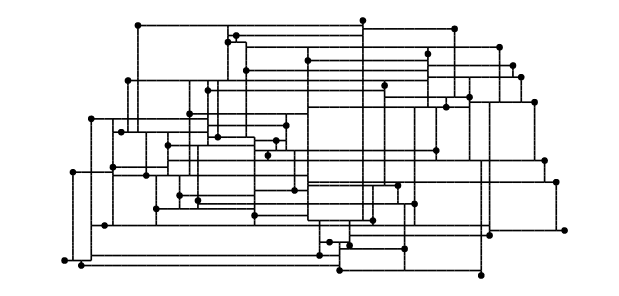
\includegraphics[width=\linewidth]{img/mn_example.png}
  \caption{A minimal Manhattan network.}
  \label{fig:mn_expamle}
\end{figure}
But in general any two directions can define the edge's possible layouts for our network.
\subsection{Minimal Manhattan networks}
A Minimal Manhattan network has obviously the same properties as a Manhattan network, but we add to them a constraint: the sum of the length of all edges (lines in the network) must be the lowest possible.

It is by using numerous approximating and/or rounding algorithms and data structures that we will ensure that what we create is a real minimal Manhattan network.

This simple constraint will totally change the way we approach the problem and how we shall solve it. By trying to find  a minimal solution we are greatly increasing the complexity of the work that will be needed to do to answer our question.

\section{First paper publish on the topic}%%%%%%%%%%%%%%%%%%%%%%%%%%%%%%%%%%
Gudmundsson, Levcopoulos and Narasimhan are three scientists that worked together in the 90's on this specific topic. Finding a Minimal Manhattan network for a given set of terminals as quick as possible was their objective. In fact at the time it wasn't known that this problem was actually NP-Hard, and required a lot of calculation to be solved.

This is why after a long work the pioneers of the MMN published two algorithms with factors 4 and 8. Knowing that this problem was bind to be difficult they emitted the conjecture that a factor 2 algorithm must exist.

And it is at this time that they opened the door to a vast community of researchers to work on the topic and also variants of this problem.

But before going deeper into the explanation we need to define the elements that we are going to work on. 

\section{Origins of the topic}%%%%%%%%%%%%%%%%%%%%%%%%%%%%%%%%%%%%%%%%%%%%%%%
The minimal Manhattan network problem was in fact formulated in 1999 by Gudmundsson, Levcopoulos and Narasimhan whom found the two approximating algorithms. 

Moreover they did conjectured the existence of an approximating algorithm of factor 2, without having any idea if they were close to find this algorithm or not. Nevertheless that this conjectured algorithm could give the solution to our problem with a cost lower than two times the optimal cost to find the optimal solution.

Actually, this algorithm was found in 2005 by my internship's mentors, Y.Vaxes and V.Chepoi, along with K.Nouioua and N.Catusse by using rounding method on a factional optimal solution, and then coupling it with a primal-dual algorithm.

Later other variants of this problem were studied, like for example the generalization of the problem to the normed plane with polygonal balls (in the l1-metric this polygon ball is a lozenge and not a always a square). And for this version of the MMN an algorithm factor 2.5 was found [2].